% =============================================================================
% main.tex — Documento final de Proyecto de Grado
% Universidad Privada del Valle — Norma DAAP 2019
%
% Motor requerido: XeLaTeX
%   Compilar con: latexmk -xelatex main.tex   (desde la raíz del repo)
% Capítulos en content/chapter-N/content.tex (índice: documento/01-estructura-capitulos.md)
% =============================================================================

\documentclass{univalle-perfil}
\addbibresource{documento.bib}

% Numeración de figuras y cuadros por capítulo (Figura 2.1, Cuadro 3.2, ...)
\counterwithin{figure}{section}
\counterwithin{table}{section}

% --- Carátula ----------------------------------------------------------------
\universidad{Universidad Privada del Valle}
\facultad{Facultad de Informática y Electrónica}
\carrera{Carrera de Licenciatura en Ingeniería de Sistemas}
\tituloTrabajo{Módulo de inteligencia predictiva del ERP ISI Mustang basado en el aprovechamiento de datos históricos operativos para anticipar desviaciones y riesgos en la gestión de proyectos de ingeniería EPC}
\modalidad{Proyecto de Grado}
\tituloOptar{Licenciatura en Ingeniería de Sistemas}
\postulante{Franco Javier Torrez Alvarado}
\tutor{Rolando Lara Sanchez}
\ciudad{Santa Cruz}
\pais{Bolivia}
\anio{2026}

\begin{document}

\makecaratula

% --- Índices (sin numerar) ---------------------------------------------------
\pagenumbering{gobble}
\tableofcontents
\listoffigures
\listoftables

% --- Cuerpo ------------------------------------------------------------------
\pagenumbering{arabic}

\section*{INTRODUCCIÓN}
\addcontentsline{toc}{section}{INTRODUCCIÓN}
% TODO: redactar al final, cuando estén los cuatro capítulos.

% Capítulo I — Marco General
% Fuente: perfil/perfil.tex (aprobado), expandido al formato de capítulo. Ver documento/02-mapeo-fuentes.md
\capitulo{1}{I}{Marco General}

\subsection{ANTECEDENTES}

\subsection{PLANTEAMIENTO DEL PROBLEMA}
\subsubsection{FORMULACIÓN DEL PROBLEMA}

\subsection{OBJETIVOS}
\subsubsection{OBJETIVO GENERAL}
\subsubsection{OBJETIVOS ESPECÍFICOS}

\subsection{JUSTIFICACIÓN}
\subsubsection{JUSTIFICACIÓN TÉCNICA}
\subsubsection{JUSTIFICACIÓN ECONÓMICA}
\subsubsection{JUSTIFICACIÓN SOCIAL}

\subsection{METODOLOGÍA}
\subsubsection{TIPO DE INVESTIGACIÓN}
\subsubsection{MÉTODO DE INVESTIGACIÓN}
\subsubsection{TÉCNICAS E INSTRUMENTOS DE INVESTIGACIÓN}
\subsubsection{POBLACIÓN Y MUESTRA}

% Capítulo II — Marco Teórico y Tecnológico
% Cada subsección se redacta a partir de su brief en documento/investigacion/ (pipeline investigador → redactor → revisor).
\capitulo{2}{II}{Marco Teórico y Tecnológico}

\subsection{SISTEMAS ERP}
\subsubsection{DEFINICIÓN Y CARACTERÍSTICAS}
\subsubsection{ERP EN EMPRESAS DE INGENIERÍA}
\subsubsection{ERP EN EL SECTOR DE PETRÓLEO, GAS Y MINERÍA}

\subsection{APRENDIZAJE AUTOMÁTICO}
\subsubsection{TIPOS DE APRENDIZAJE}

El aprendizaje automático (\textit{machine learning}) es la rama de la inteligencia artificial que estudia los algoritmos capaces de mejorar su desempeño de manera automática a partir de la experiencia. \textcite{Mitchell1997} lo formaliza con tres elementos: se dice que un programa aprende de una experiencia $E$ respecto de una clase de tareas $T$ y una medida de desempeño $P$ si su desempeño en $T$, medido por $P$, mejora con $E$. Trasladada al presente proyecto, la experiencia es el histórico operativo de más de diez años de ISI Mustang, la tarea es anticipar desviaciones en sus proyectos y la medida de desempeño son las métricas que se describen en la subsección siguiente.

La forma en que esa experiencia se presenta al algoritmo define los paradigmas clásicos del campo. \textcite{Geron2022} organiza los sistemas de aprendizaje automático según la supervisión que reciben durante el entrenamiento en tres familias: supervisado, no supervisado y por refuerzo. En el aprendizaje supervisado cada observación de entrenamiento viene acompañada de la respuesta correcta, la etiqueta o valor objetivo, y el algoritmo aprende una función que asocia las entradas con esa salida para predecirla sobre observaciones nuevas \parencite{Hastie2009}. En el aprendizaje no supervisado no existe tal respuesta: el algoritmo recibe únicamente las entradas y busca estructura en ellas, como grupos de observaciones similares o direcciones de mayor variabilidad \parencite{James2021}. El aprendizaje por refuerzo, por último, no parte de un conjunto de datos fijo sino de un agente que interactúa con un entorno y ajusta su comportamiento según las recompensas que recibe \parencite{Mitchell1997}.

Dentro del aprendizaje supervisado, la naturaleza de la variable de salida distingue dos tipos de problema. Cuando la salida es cuantitativa (un monto, una duración, un porcentaje) se habla de regresión; cuando es cualitativa o categórica (una clase entre un conjunto finito) se habla de clasificación \parencite{Hastie2009, James2021}. La distinción no es solo nominal: determina qué algoritmos son aplicables, qué función de pérdida se optimiza y con qué métricas se evalúa el resultado.

Los tres casos de uso del módulo predictivo se ubican en el paradigma supervisado, porque el histórico de la empresa ya contiene el resultado de cada proyecto cerrado: se conoce cuánto costó respecto de lo presupuestado, cuándo se cerró respecto de la fecha comprometida y cómo evolucionaron sus certificaciones frente a lo planificado. La predicción de desviación en certificaciones es un problema de clasificación, mientras que la estimación del sobrecosto y del retraso en la fecha de cierre son problemas de regresión. El aprendizaje no supervisado y el aprendizaje por refuerzo quedan fuera del alcance del proyecto.

\subsubsection{APRENDIZAJE SUPERVISADO}

Formalmente, el aprendizaje supervisado parte de un conjunto de entrenamiento compuesto por pares $(x_i, y_i)$, donde $x_i$ es un vector de variables predictoras y $y_i$ la respuesta observada, y busca una función $f$ tal que $f(x)$ aproxime a $y$ con el menor error posible sobre observaciones que no participaron del entrenamiento \parencite{Hastie2009}. Esta última condición es la que separa aprender de memorizar. \textcite{James2021} distinguen el error de entrenamiento, que mide el ajuste sobre los datos vistos, del error de prueba, que mide la capacidad de generalizar; un modelo puede reducir el primero indefinidamente aumentando su complejidad, pero a partir de cierto punto el segundo empieza a crecer. Ese fenómeno es el sobreajuste, y se explica por el compromiso entre sesgo y varianza: los modelos simples tienen sesgo alto porque no capturan la estructura de los datos, mientras que los modelos muy flexibles tienen varianza alta porque se ajustan al ruido de la muestra particular con la que fueron entrenados \parencite{Hastie2009, James2021}.

Como el error de prueba no puede calcularse sobre los datos de entrenamiento, se requiere un procedimiento para estimarlo. La práctica básica consiste en separar una parte de los datos como conjunto de prueba, que se reserva y solo se usa al final para evaluar el modelo elegido \parencite{Geron2022}. Para seleccionar entre modelos o ajustar hiperparámetros sin contaminar ese conjunto se emplea la validación cruzada de $k$ particiones (\textit{k-fold}): los datos de entrenamiento se dividen en $k$ bloques, el modelo se entrena $k$ veces dejando fuera un bloque distinto en cada corrida y el error se promedia sobre las $k$ evaluaciones \parencite{James2021}. En un estudio empírico de referencia, \textcite{Kohavi1995} concluye que la validación cruzada estratificada de diez particiones es el mejor método para selección de modelos, incluso cuando la capacidad de cómputo permite usar más particiones, y advierte que la variante \textit{leave-one-out}, aunque casi insesgada, tiene alta varianza y produce estimaciones poco confiables. La estratificación conserva en cada bloque la proporción de clases del conjunto completo, lo que importa cuando una de las clases es minoritaria.

La evaluación del modelo depende del tipo de problema. En clasificación, las medidas usuales derivan de la matriz de confusión, que cruza la clase real con la clase predicha y separa los verdaderos positivos (VP), verdaderos negativos (VN), falsos positivos (FP) y falsos negativos (FN) \parencite{Sokolova2009, Geron2022}. A partir de ella se calculan la exactitud (proporción de aciertos sobre el total), la precisión (proporción de positivos predichos que realmente lo son), la sensibilidad o \textit{recall} (proporción de positivos reales que el modelo detecta) y la medida F1, media armónica de las dos anteriores. \textcite{Sokolova2009} muestran que estas medidas no reaccionan igual ante cambios en la distribución de clases: la exactitud puede ser alta en un conjunto desbalanceado aunque el modelo ignore la clase minoritaria, razón por la cual conviene reportarlas juntas. En regresión, el punto de partida es el error cuadrático medio (MSE), promedio de las diferencias al cuadrado entre valor observado y predicho \parencite{James2021}; su raíz, el RMSE, se expresa en las unidades de la variable y penaliza con más fuerza los errores grandes, mientras que el error absoluto medio (MAE) promedia las diferencias en valor absoluto y es menos sensible a valores extremos. \textcite{Chai2014} sostienen que el RMSE es más apropiado cuando se espera que los errores sigan una distribución gaussiana y que, en general, evaluar un modelo requiere una combinación de métricas y no una sola. A estas se suma el coeficiente de determinación $R^2$, que expresa la proporción de la variabilidad de la respuesta que el modelo explica y permite comparar el ajuste entre variables de distinta escala. El cuadro~\ref{tab:metricas-supervisado} resume las métricas y su uso en el proyecto.

\begin{table}[H]
  \centering
  \caption{Métricas de evaluación de modelos supervisados y su uso en el proyecto}\label{tab:metricas-supervisado}
  \begin{tabular}{@{}>{\RaggedRight\arraybackslash}p{0.18\textwidth}>{\RaggedRight\arraybackslash}p{0.33\textwidth}>{\RaggedRight\arraybackslash}p{0.43\textwidth}@{}}
    \toprule
    \textbf{Métrica} & \textbf{Qué mide} & \textbf{Uso en el proyecto} \\
    \midrule
    \multicolumn{3}{@{}l}{\textit{Clasificación}} \\
    Matriz de confusión & Cruce de clase real y clase predicha (VP, VN, FP, FN) & Base de las demás métricas; muestra qué tipo de error comete el clasificador de desviación en certificaciones \\
    Exactitud & $(\mathrm{VP}+\mathrm{VN})/\mathrm{total}$ & Referencia general; insuficiente si las clases están desbalanceadas \\
    Precisión & $\mathrm{VP}/(\mathrm{VP}+\mathrm{FP})$ & Proporción de alertas de desviación que son correctas \\
    Sensibilidad & $\mathrm{VP}/(\mathrm{VP}+\mathrm{FN})$ & Proporción de desviaciones reales que el modelo detecta \\
    F1 & Media armónica de precisión y sensibilidad & Resumen único cuando ambas importan \\
    \midrule
    \multicolumn{3}{@{}l}{\textit{Regresión}} \\
    RMSE & Raíz del promedio de errores al cuadrado & Error en unidades de la variable; penaliza sobrecostos o retrasos grandes mal estimados \\
    MAE & Promedio de errores en valor absoluto & Error típico esperado, robusto a valores extremos \\
    $R^2$ & Proporción de la variabilidad explicada por el modelo & Comparación del ajuste entre el modelo de sobrecosto y el de retraso \\
    \bottomrule
  \end{tabular}
  \fuente{Elaboración propia.}
\end{table}

Estas definiciones fijan el protocolo de evaluación del módulo predictivo: el clasificador de desviación en certificaciones se evaluará con exactitud, precisión, sensibilidad, F1 y matriz de confusión; los regresores de sobrecosto y de retraso en la fecha de cierre, con RMSE, MAE y $R^2$; y en los tres casos la selección de hiperparámetros se hará con validación cruzada estratificada sobre el conjunto de entrenamiento, reservando un conjunto de prueba independiente para la evaluación final.

\subsubsection{ALGORITMOS DE APRENDIZAJE SUPERVISADO: GRADIENT BOOSTING Y XGBOOST}

El aprendiz base de los algoritmos que usa este proyecto es el árbol de decisión. Un árbol particiona recursivamente el espacio de las variables predictoras mediante reglas binarias del tipo «presupuesto mayor que cierto umbral» y asigna a cada región resultante una predicción constante: la clase mayoritaria en clasificación o el promedio de las respuestas en regresión \parencite{Hastie2009, James2021}. El procedimiento CART formalizado por \textcite{Breiman1984} es el que implementan Scikit-learn y las bibliotecas de \textit{boosting}. Los árboles son fáciles de interpretar y admiten sin transformación previa variables numéricas y categóricas, pero un árbol aislado tiene alta varianza (pequeños cambios en los datos producen árboles muy distintos) y su capacidad predictiva suele ser inferior a la de otros métodos \parencite{James2021}.

Los métodos de ensamble corrigen esa debilidad combinando muchos árboles, con dos estrategias distintas. En el \textit{bagging} y los bosques aleatorios de \textcite{Breiman2001}, los árboles se entrenan en paralelo sobre remuestreos de los datos y sus predicciones se promedian, lo que reduce la varianza. En el \textit{boosting}, en cambio, los árboles se construyen de forma secuencial: cada nuevo árbol se ajusta a lo que los anteriores todavía no explican, de modo que el ensamble mejora por etapas \parencite{Hastie2009, James2021}. \textcite{Friedman2001} dio a esta idea su formulación general al plantear la estimación de la función como un problema de optimización numérica en el espacio de funciones: en cada etapa se ajusta un árbol de regresión al gradiente negativo de la función de pérdida evaluada sobre el modelo acumulado, lo que equivale a un descenso por gradiente en el que cada paso es un árbol. El marco admite distintas funciones de pérdida (mínimos cuadrados, desviación absoluta o Huber para regresión, y verosimilitud logística para clasificación), de modo que el mismo algoritmo sirve para los problemas de regresión y de clasificación del proyecto. Sus hiperparámetros principales son el número de árboles, la tasa de aprendizaje o \textit{shrinkage}, que reduce la contribución de cada árbol, y la profundidad de los árboles, que controla el orden de las interacciones entre variables \parencite{James2021}; el submuestreo de observaciones en cada etapa agrega una regularización adicional \parencite{Hastie2009}.

XGBoost es la implementación de \textit{gradient boosting} de árboles que utiliza el proyecto. \textcite{Chen2016} la presentan como un sistema escalable, ampliamente usado para obtener resultados de vanguardia en competencias de aprendizaje automático, y describen sus aportes: un algoritmo consciente de la dispersión (\textit{sparsity-aware}) para datos dispersos, un esquema de cuantiles ponderados para construir árboles de forma aproximada, y optimizaciones de caché, compresión y particionado que le permiten escalar a miles de millones de ejemplos con menos recursos que otros sistemas. En el diseño del módulo predictivo se prevé aprovechar el tratamiento de valores ausentes que ofrece la biblioteca, dado que el histórico del ERP presenta registros incompletos, y ajustar mediante validación cruzada tanto los hiperparámetros del \textit{boosting} ya mencionados como los parámetros de regularización que XGBoost expone sobre la complejidad de los árboles.

La elección de \textit{gradient boosting} frente a alternativas más recientes se apoya en evidencia sobre datos tabulares. \textcite{Grinsztajn2022} compararon modelos de árboles y redes neuronales profundas sobre 45 conjuntos de datos tabulares y concluyeron que los primeros siguen siendo el estado del arte en conjuntos de tamaño medio, del orden de diez mil observaciones, aun sin considerar su ventaja en velocidad; atribuyen el resultado a sesgos inductivos de los árboles, como la robustez frente a variables no informativas y la capacidad de aprender funciones irregulares, que las redes no comparten. \textcite{ShwartzZiv2022} llegaron a la misma conclusión al enfrentar XGBoost con modelos profundos diseñados específicamente para datos tabulares: XGBoost los superó incluso en los conjuntos de datos usados por los artículos que los proponían y requirió mucho menos ajuste. Ambos resultados describen el escenario del proyecto (datos tabulares de tamaño medio extraídos de un ERP, un solo desarrollador y un plazo acotado) y justifican adoptar XGBoost, integrado con la API de Scikit-learn \parencite{Pedregosa2011}, como algoritmo para los tres casos de uso.

\subsubsection{FEATURE ENGINEERING}

La ingeniería de características (\textit{feature engineering}) es el conjunto de operaciones que transforman los datos crudos en las variables predictoras que recibe el modelo. \textcite{Kuhn2019} la sitúan dentro del proceso de modelado predictivo, junto con la división de datos, el remuestreo, el ajuste de hiperparámetros y la evaluación, y sostienen que la representación de los predictores condiciona el desempeño tanto como la elección del algoritmo. \textcite{Geron2022} muestra el mismo proceso desde la práctica con Scikit-learn: limpieza, codificación de variables categóricas, escalado y encadenamiento de esas transformaciones en \textit{pipelines} que se ajustan únicamente con datos de entrenamiento, para evitar que información del conjunto de prueba se filtre al modelo.

Tres grupos de técnicas son relevantes para este proyecto. El primero es la codificación de predictores categóricos, como el cliente, el tipo de proyecto o el rubro: \textcite{Kuhn2019} describen la codificación \textit{one-hot} o por variables indicadoras, el agrupamiento de categorías poco frecuentes y las codificaciones supervisadas, que reemplazan cada categoría por un estadístico de la respuesta, útiles cuando la variable tiene muchos niveles. El segundo es la transformación de predictores numéricos, que incluye el centrado y escalado, las transformaciones para corregir asimetría y la discretización en intervalos. El tercero, y el más sensible en un histórico operativo, es el manejo de datos faltantes: los mismos autores recomiendan visualizar primero el patrón de ausencia, y luego decidir entre eliminar observaciones o variables, imputar los valores o emplear modelos tolerantes a faltantes. Esta última opción se conecta con los defectos de calidad del ERP identificados en el análisis de datos y con la capacidad de XGBoost mencionada en la subsección anterior.

La selección de variables completa el proceso. \textcite{Guyon2003} le atribuyen tres objetivos: mejorar el desempeño del predictor, obtener modelos más rápidos y económicos, y comprender mejor el proceso que generó los datos. \textcite{Kuhn2019} clasifican los métodos en filtros, que evalúan cada variable de forma independiente del modelo, y envolventes (\textit{wrappers}), que buscan subconjuntos de variables evaluando el modelo sobre cada candidato mediante estrategias voraces, como la eliminación recursiva, o globales; y advierten que, si la selección se realiza fuera del esquema de remuestreo, la estimación del error queda sesgada de forma optimista.

Como decisión de diseño del proyecto, la ingeniería de características se implementa en la capa Gold del pipeline de datos con Polars, y construye para cada proyecto un vector de variables a partir de sus atributos maestros y de agregados calculados sobre sus registros transaccionales a una fecha de corte, como totales y proporciones acumuladas. Un requisito propio de este caso es que las mismas variables deben poder calcularse tanto desde el histórico MySQL del portal anterior, que alimenta el entrenamiento, como desde el ERP nuevo en PostgreSQL, sobre el que se hará la inferencia; sin ese mapeo común, un modelo entrenado con una fuente no puede aplicarse a la otra.


\subsection{INGENIERÍA DE DATOS}
\subsubsection{PROCESOS ETL Y ELT}
\subsubsection{ARQUITECTURA MEDALLION (BRONZE, SILVER, GOLD)}
\subsubsection{CALIDAD DE DATOS}

\subsection{ANALÍTICA PREDICTIVA}
\subsubsection{DEFINICIÓN Y APLICACIONES}
\subsubsection{ANALÍTICA PREDICTIVA EN GESTIÓN DE PROYECTOS}
\subsubsection{PREDICCIÓN DE DESVIACIONES Y COSTOS}

\subsection{GESTIÓN DE PROYECTOS EPC}
\subsubsection{DEFINICIÓN Y CARACTERÍSTICAS}
\subsubsection{CERTIFICACIONES Y CONTROL DE AVANCE}
\subsubsection{DESVIACIONES PRESUPUESTARIAS Y DE CRONOGRAMA}

\subsection{INGENIERÍA DE SOFTWARE}
\subsubsection{PROCESO DE DESARROLLO DE SOFTWARE}
\subsubsection{METODOLOGÍA DE DESARROLLO ITERATIVA E INCREMENTAL}
\subsubsection{ARQUITECTURA DE SOFTWARE POR CAPAS}

\subsection{TECNOLOGÍAS DEL STACK DE DESARROLLO}
\subsubsection{PYTHON Y SU ECOSISTEMA ML}
\subsubsection{DUCKDB Y POLARS}
\subsubsection{FASTAPI COMO MICROSERVICIO}
\subsubsection{NESTJS Y ANGULAR}

\subsection{GESTIÓN DE IDENTIDAD Y ACCESO}
\subsubsection{OAUTH 2.0 Y OPENID CONNECT}
\subsubsection{KEYCLOAK}

\subsection{MODEL CONTEXT PROTOCOL (MCP)}
\subsubsection{DEFINICIÓN Y ARQUITECTURA}
\subsubsection{INTEGRACIÓN DE SISTEMAS EMPRESARIALES CON MODELOS DE LENGUAJE}

\subsection{INTELIGENCIA DE NEGOCIOS}
\subsubsection{DEFINICIÓN Y REPORTES DESCRIPTIVOS}
\subsubsection{POWER BI}

% Capítulo III — Análisis y Diseño del Sistema Propuesto
% Hallazgos abiertos al redactar: documento/16-hallazgos-cap3.md. Decisiones: documento/12-necesidades-cap3.md.
\capitulo{3}{III}{Análisis y Diseño del Sistema Propuesto}

% 3.1 — fuente: dump del MySQL de producción del portal anterior (documento/referencias/isidump.sql, 2026-09-17), consultas SQL
% sobre una copia local; cifras y consultas resumidas en documento/12-necesidades-cap3.md (H1–H9) y documento/16-hallazgos-cap3.md.
% Las planillas Excel de control todavía no están disponibles: cuando lleguen se agregan a 3.1.1 y se recalculan las cifras.
\subsection{ANÁLISIS DE DATOS HISTÓRICOS}

Este análisis responde al segundo objetivo específico: determinar, con los datos y no con supuestos, si el histórico permite construir los tres casos de uso del módulo predictivo, con qué variables y sobre cuántos casos. Se realizó sobre una copia completa de la base de datos de producción del portal anterior, exportada en septiembre de 2026 y cargada en un servidor MySQL local, sin conexión con el sistema en operación. Las cifras de esta sección provienen de consultas SQL sobre esa copia; el pipeline de la sección 3.4 las reproduce con DuckDB y Polars. Las planillas Excel de control de proyectos que la empresa lleva fuera del sistema no estaban disponibles al cierre de este análisis, por lo que las cifras corresponden solo a la base de datos del portal.

\subsubsection{EXPLORACIÓN Y CARACTERIZACIÓN DE LAS FUENTES DE DATOS}

La base del portal contiene 163 tablas con datos. La mayoría son catálogos, permisos y tablas de recursos humanos; estas últimas, con remuneraciones y datos personales, se excluyeron del análisis desde el inicio (RNF-03). La tabla~\ref{tab:fuentes-historico} resume las tablas de la base que describen la ejecución de los proyectos. No se encontró una tabla de certificaciones como tal: las certificaciones son ítems del flujo de caja de cada proyecto, identificados por su rubro, con fecha planificada y fecha real.

\begin{tabla}[H]
  \centering
  \caption{Tablas del portal anterior usadas en el análisis}\label{tab:fuentes-historico}
  \small
  \begin{tblr}{colspec={X[1.04,l] X[1.82,l] X[0.44,r] X[0.7,l]}}
    \textbf{Tabla} & \textbf{Contenido} & \textbf{Filas} & \textbf{Período} \\
    \texttt{act\_proyecto} & Maestro de centros de costo: fechas, plazo, monto de la orden de compra, presupuesto de costo por rubro, horas planificadas, margen proyectado & 292 & 2003--2026 \\
    \texttt{adicionales} & Ampliaciones de alcance con su monto y costo presupuestado & 237 & 2005--2020 \\
    \texttt{gpre} & Flujo de caja vigente por ítem; las certificaciones son los rubros \texttt{WI001} (orden de compra) y \texttt{WA001} (adicionales) & 10\,872 & 2008--2027 \\
    \texttt{gprepublicadomensual} & Foto mensual del flujo de caja publicado & 170\,225 & 2013--2020 \\
    \texttt{gpreeventos} & Registro de cambios al flujo de caja & 47\,896 & 2013--2020 \\
    \texttt{gpdir} & Asientos contables por centro de costo: débito como costo y crédito como ingreso & 81\,307 & 2008--2025 \\
    \texttt{horas}, \texttt{horasctroctos} & Horas diarias por persona y su asignación a centros de costo & 310\,137 & 2005--2024 \\
    \texttt{rq} & Requisiciones de compra & 6\,165 & 2006--2026 \\
    \texttt{viaticos} & Pedidos de viáticos & 3\,713 & 2011--2026 \\
    \texttt{propuestas} & Oportunidades comerciales, con el sector industrial & 844 & 2013--2026 \\
  \end{tblr}
  \fuente{Elaboración propia, 2026, en base a la base de datos del portal anterior.}
\end{tabla}

El universo de análisis son los centros de costo cerrados de tipo proyecto (prefijos \texttt{O} y \texttt{C}) y servicio (prefijo \texttt{S}): 248 centros de costo, 175 de proyecto u operación, 57 de servicio y 16 de consultoría, con fechas de inicio entre 2003 y 2026. La figura~\ref{fig:proyectos-anio} muestra su distribución por año de inicio y, para cada año, cuántos tienen un flujo de caja con certificaciones. El hallazgo central es que el flujo de caja del portal se usó para planificar y registrar certificaciones solo entre 2010 y 2018: antes de 2010 casi no hay certificaciones registradas, y a partir de 2019 los proyectos siguen teniendo costos contables, pero no certificaciones.

\begin{figure}[H]
\centering
\caption{Centros de costo cerrados por año de inicio}\label{fig:proyectos-anio}
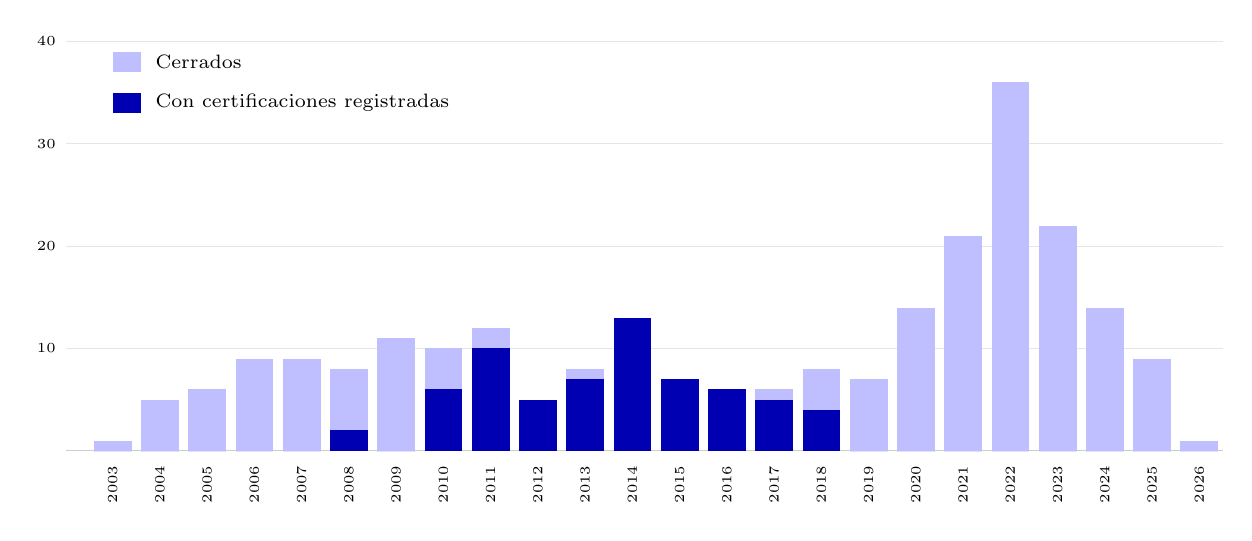
\begin{tikzpicture}[x=0.6cm, y=0.13cm]
  \draw[gray!40] (0,0) -- (24.5,0);
  \foreach \v in {10,20,30,40} {
    \draw[gray!20] (0,\v) -- (24.5,\v);
    \node[font=\tiny, anchor=east] at (0,\v) {\v};
  }
  \foreach \i/\y/\c/\k in {1/2003/1/0, 2/2004/5/0, 3/2005/6/0, 4/2006/9/0, 5/2007/9/0, 6/2008/8/2, 7/2009/11/0, 8/2010/10/6, 9/2011/12/10, 10/2012/5/5, 11/2013/8/7, 12/2014/13/13, 13/2015/7/7, 14/2016/6/6, 15/2017/6/5, 16/2018/8/4, 17/2019/7/0, 18/2020/14/0, 19/2021/21/0, 20/2022/36/0, 21/2023/22/0, 22/2024/14/0, 23/2025/9/0, 24/2026/1/0} {
    \fill[blue!25] (\i-0.4,0) rectangle (\i+0.4,\c);
    \fill[blue!70!black] (\i-0.4,0) rectangle (\i+0.4,\k);
    \node[font=\tiny, rotate=90, anchor=east] at (\i,-0.5) {\y};
  }
  \fill[blue!25] (1,37) rectangle (1.6,39); \node[font=\scriptsize, anchor=west] at (1.7,38) {Cerrados};
  \fill[blue!70!black] (1,33) rectangle (1.6,35); \node[font=\scriptsize, anchor=west] at (1.7,34) {Con certificaciones registradas};
\end{tikzpicture}
\fuente{Elaboración propia, 2026, en base a la base de datos del portal anterior.}
\end{figure}

La calidad de los datos se evaluó con las dimensiones de la sección 2.3, respecto de su uso en el módulo predictivo (cuadro~\ref{tab:calidad-historico}). Dos defectos condicionan el diseño. El primero es que el flujo de caja sobrescribe la fecha planificada de cada certificación cuando se replanifica, de modo que comparar la fecha planificada vigente con la real no mide ningún desvío; la fecha original solo puede recuperarse de las fotos mensuales, que existen desde julio de 2013. El segundo es que la fecha de cierre de los proyectos es administrativa: ocho fechas concentran cinco o más cierres cada una, y seis proyectos figuran cerrados antes de su inicio. Tampoco se registraron causas de desviación: las columnas previstas para la causa y la mitigación están vacías, lo que descarta la hipótesis planteada en la sección 1.4 de que las causas documentadas pudieran usarse como parte del conjunto de datos.

\begin{table}[H]
  \centering
  \caption{Calidad del histórico del portal anterior por dimensión}\label{tab:calidad-historico}
  \small
  \begin{tblr}{colspec={X[0.49,l] X[1.63,l] X[0.88,l]}}
    \textbf{Dimensión} & \textbf{Hallazgo} & \textbf{Efecto en el módulo} \\
    Exactitud & Fecha planificada de certificación sobrescrita al replanificar; fecha de cierre administrativa; en 28 de 60 proyectos la última certificación real coincide exactamente con la planificada original & Etiquetas de desvío y de retraso \\
    Completitud & Sin causas de desviación; certificaciones solo en 2010--2018; antes de 2020, solo entre un cuarto y un tercio de las horas cargadas pueden asignarse a un centro de costo; sector industrial registrado solo desde 2020 & Tamaño del conjunto y variables disponibles \\
    Consistencia & El ingreso contable convertido a dólares concilia con la orden de compra más adicionales (diferencia menor al 15\,\%) en 113 proyectos; desde 2020 el rubro contable de los asientos está vacío en la mayoría de los casos & Etiqueta de sobrecosto \\
    Unicidad & Siete códigos de centro de costo aparecen dos veces en el maestro de proyectos & Deduplicación en Silver \\
    Validez & Tipo de cambio igual a uno en casi todos los asientos de 2008 a 2010 y en la mayoría de los de 2012, con moneda ambigua; plazos de ejecución de 1 a 7 días en proyectos de meses; cierre anterior al inicio; texto con codificación dañada & Filtros y variables excluidas \\
    Oportunidad & No evaluada: el portal no registra cuándo se cargó cada dato respecto del evento & --- \\
  \end{tblr}
  \fuente{Elaboración propia, 2026, en base a la base de datos del portal anterior y de la sección 2.3.}
\end{table}

\subsubsection{IDENTIFICACIÓN DE VARIABLES PREDICTORAS}

Una variable candidata debe cumplir dos condiciones: estar disponible en el histórico con completitud suficiente y tener equivalente en el ERP nuevo, donde se realiza la inferencia. La tabla~\ref{tab:variables-candidatas} evalúa las candidatas sobre los 75 centros de costo cerrados que iniciaron entre 2010 y 2018, el período en que existen las etiquetas.

\begin{tabla}[H]
  \centering
  \caption{Variables predictoras candidatas}\label{tab:variables-candidatas}
  \footnotesize
  \begin{tblr}{colspec={X[1.19,l] X[0.62,r] X[0.97,l] X[1.23,l]}}
    \textbf{Variable} & \textbf{Completitud 2010--2018} & \textbf{Equivalente en el ERP nuevo} & \textbf{Decisión} \\
    Monto vendido y presupuesto de costo por bolsa & 97--99\,\% & Líneas de presupuesto de línea base & Se usa \\
    Horas planificadas & 94\,\% & Horas de la bolsa de servicios & Se usa \\
    Margen bruto proyectado & 87\,\% & Derivable del vendido & Se usa \\
    Ampliaciones de alcance & 61\,\% con adicionales & Crecimiento del vendido desde la línea base inicial & Se usa como crecimiento del vendido \\
    Replanificaciones del flujo de caja & 94\,\% & Bitácora del presupuesto & Se usa \\
    Costo ejecutado acumulado & 100\,\% (83\,\% concilia) & Ejecutado del presupuesto & Se usa \\
    Certificado acumulado frente a planificado & 84\,\% & Certificaciones & Se usa \\
    Requisiciones y viáticos & 79 y 66\,\% & Órdenes de compra y rendiciones & Se usa; ausencia equivale a cero \\
    Horas cargadas & 99\,\% con horas, cobertura parcial & Horas aprobadas & Se usa con cautela; se evalúa su aporte \\
    Tipo de centro de costo & 100\,\% & Tipo de centro de costo & Se usa \\
    Plazo de ejecución registrado & 100\,\% & Fechas de vigencia & Se descarta: valores no comparables \\
    Sector industrial & 0\,\% & Mercado de la propuesta & Se descarta en el entrenamiento \\
    Cliente & No resoluble & Cliente & Se descarta: los identificadores no existen en las tablas de clientes \\
    Avance físico & No existe & No existe & Se descarta \\
  \end{tblr}
  \fuente{Elaboración propia, 2026, en base a la base de datos del portal anterior y del esquema del ERP nuevo.}
\end{tabla}

Las variables retenidas describen el proyecto por su tamaño, la composición de su presupuesto, la estabilidad de su plan y el ritmo de su ejecución económica. Ninguna mide el avance físico, que el portal no registraba y el ERP nuevo tampoco define (sección 3.2); el avance se aproxima con el tiempo transcurrido, el costo ejecutado y lo certificado frente a lo planificado. Como las variables se calculan a una fecha de corte (sección 3.4), cada una se reconstruye solo con los registros fechados hasta ese corte.

\subsubsection{DEFINICIÓN DE CASOS DE USO PREDICTIVOS}

Los tres casos de uso se definen con reglas de etiquetado explícitas, aplicables por igual al histórico y al ERP nuevo. Los umbrales siguen el semáforo del ERP: una desviación desfavorable de hasta 5\,\% es verde, de hasta 10\,\% amarilla y mayor, roja (REQ~12.11); para las certificaciones, el requerimiento de la empresa fija en 10\,\% el desvío que exige causa y mitigación (REQ~13.9). La tabla~\ref{tab:casos-uso} resume el resultado.

\paragraph{Desviación en certificaciones}

La unidad es la certificación. Se considera desviada si se certificó después de su fecha planificada original por más del 10\,\% del plazo planificado del proyecto, o por un monto inferior en más del 10\,\% al planificado originalmente. El plazo planificado es el tiempo entre el inicio del proyecto y su última certificación planificada original. Con la fecha original tomada de las fotos mensuales, se obtienen 831 certificaciones con fecha real de 65 proyectos, de las cuales 134 (16\,\%) están desviadas. La cifra está sesgada a la baja para los proyectos iniciados antes de julio de 2013, cuyo plan ya podía estar modificado cuando se tomó la primera foto: entre los 42 proyectos iniciados después, 113 de 389 certificaciones (29\,\%) están desviadas.

\paragraph{Sobrecosto}

La unidad es el proyecto. El sobrecosto es el costo ejecutado al cierre respecto del vendido, en porcentaje. En el histórico, el costo ejecutado se toma de los asientos contables convertidos a dólares, y el vendido, del presupuesto de costo más los adicionales. Solo se usan los proyectos cuyo ingreso contable concilia con la orden de compra más adicionales, como control de que la conversión de moneda es correcta: 113 proyectos. De ellos, 61 cerraron por debajo del vendido, 13 lo superaron hasta en un 10\,\% y 39 en más del 10\,\%. Diez superan el 100\,\%, valores que se revisan como posibles errores de registro antes del entrenamiento.

\paragraph{Retraso en la fecha de cierre}

La unidad es el proyecto. Como la fecha de cierre registrada es administrativa, el fin real se toma de la última certificación real y el fin planificado, de la última certificación planificada en la primera foto mensual. El retraso se expresa como porcentaje del plazo planificado. Con proyectos de al menos treinta días de plazo planificado se obtienen 60 casos: 17 (28\,\%) con retraso mayor al 10\,\%, 6 con retraso de hasta 10\,\% y 37 terminados en plazo o antes. En 28 de ellos la fecha real coincide exactamente con la planificada, lo que puede reflejar un plazo cumplido o una fecha real cargada igual a la planificada; esa ambigüedad se trata como limitación.

\begin{tabla}[H]
  \centering
  \caption{Casos de uso predictivos y tamaño de sus conjuntos de datos}\label{tab:casos-uso}
  \small
  \begin{tblr}{colspec={X[1.1,l] X[0.76,l] X[0.93,l] X[1.1,l] X[1.1,l]}}
    \textbf{Caso de uso} & \textbf{Unidad} & \textbf{Tipo de problema} & \textbf{Casos con etiqueta} & \textbf{Casos desfavorables} \\
    Desviación en certificaciones & Certificación & Clasificación & 831 de 65 proyectos & 134 desviadas (16\,\%) \\
    Sobrecosto & Proyecto & Regresión & 113 & 39 sobre 10\,\% (35\,\%) \\
    Retraso en la fecha de cierre & Proyecto & Regresión & 60 & 17 sobre 10\,\% (28\,\%) \\
  \end{tblr}
  \fuente{Elaboración propia, 2026, en base a la base de datos del portal anterior.}
\end{tabla}

Los tamaños confirman la advertencia de la sección 2.2: el histórico reúne cientos de casos para las certificaciones y apenas decenas de proyectos para los otros dos casos de uso. Esto justifica dos decisiones del diseño. La primera es modelar la desviación en certificaciones por certificación y no por proyecto, porque es la única unidad con volumen suficiente. La segunda es observar cada proyecto en varias fechas de corte y validar agrupando por proyecto (sección 3.4), para aprovechar los pocos proyectos sin sobrestimar el desempeño. El tamaño reducido de los conjuntos de sobrecosto y retraso es la principal limitación del módulo predictivo; las planillas de control, si cubren los proyectos posteriores a 2018, son la vía para ampliarlos.


% 3.2 — fuentes: manual del portal anterior (erp-isi-mustang/docs/old-manual/manual.md y 05-proyectos.md),
% requerimiento vigente de la empresa (docs/documentation/complete/02-base-URS-TO-BE.md, citado como REQ) y código de
% erp-isi-mustang y portal-erp (main, verificado el 2026-09-17). Los docs AS-IS de docs/documentation/ están desactualizados: no usar.
\subsection{ANÁLISIS DE PROCESOS DEL PORTAL ANTERIOR}

Este análisis responde al primer objetivo específico: identificar qué procesos del portal anterior faltan en el ERP nuevo y qué defectos afectan la calidad de los datos. Parte de dos fuentes. La primera es el manual de usuario del Portal ISIMustang Bolivia \parencite{ISIMustang2020Manual}, publicado por la empresa en 2020 como un blog en \url{https://manualportalbolivia.blogspot.com/}, con una entrada por módulo, que describe cada proceso tal como lo operan los usuarios. La segunda es el código fuente del ERP nuevo, revisado en septiembre de 2026, contra el que se verificó el estado de cada proceso. La documentación técnica del ERP no se usó para establecer ese estado porque, en varios puntos, describe brechas que el código ya había resuelto. Las decisiones de la empresa sobre cómo debe funcionar cada proceso se toman del relevamiento de requerimientos que la empresa consolidó en agosto de 2026 \parencite{ISIMustang2026Requerimientos}, citado en adelante como REQ seguido del apartado.

\subsubsection{RELEVAMIENTO DE PROCESOS DEL PORTAL ANTERIOR}

El manual organiza el portal en módulos de horas, requisiciones y compras, viáticos, proyectos, áreas de estructura y permisos. Los cuadros~\ref{tab:procesos-portal} y~\ref{tab:procesos-portal-gestion} listan sus procesos y su estado en el ERP nuevo, con cuatro valores: \emph{implementado}, cuando el ERP nuevo cubre el proceso; \emph{parcial}, cuando lo cubre con una diferencia que afecta sus datos; \emph{reemplazado}, cuando la empresa decidió resolverlo de otro modo; y \emph{fuera de alcance}.

\begin{table}[H]
  \centering
  \caption{Procesos operativos del portal anterior y su estado en el ERP nuevo}\label{tab:procesos-portal}
  \small
  \begin{tblr}{colspec={X[1.3,l] X[0.44,l] X[0.61,l] X[1.65,l]}}
    \textbf{Proceso del portal} & \textbf{Manual} & \textbf{Estado} & \textbf{En el ERP nuevo} \\
    Carga de horas por centro de costo y tarea & 01 & Implementado & Borrador, envío y aprobación; horas de oficina y de campo, equivalentes a las HHC y PEMC del portal \\
    Consulta de horas por persona o proyecto & 04, 05.4, 06.3 & Implementado & Listados filtrables por centro de costo y por persona \\
    Pedido de requisición con aprobación & 02 & Implementado & Requisición contra centro de costo y bolsa, con motor de aprobaciones \\
    Administración de requisiciones y emisión de la orden de compra & 02.1 & Parcial & Órdenes de compra con proveedor y recepción parcial; no registran la factura del proveedor, por lo que el ejecutado de compras se toma de la orden emitida \\
    Pedido y administración de viáticos & 03, 03.2 & Implementado & Solicitud, aprobación del responsable y pago del anticipo por Compras \\
    Política de viáticos: topes de gasto y plazo de rendición & 03.1 & Reemplazado & Sin topes ni plazos formales (REQ~11.3) \\
    Rendición de viáticos & 03.3 & Implementado & Rendición en el sistema, con líneas en distintas monedas convertidas por separado; en el portal era una planilla externa \\
  \end{tblr}
  \fuente{Elaboración propia, 2026, en base a \textcite{ISIMustang2020Manual} y al código del ERP nuevo.}
\end{table}

\begin{table}[H]
  \centering
  \caption{Procesos de gestión de proyectos y estructura del portal anterior y su estado en el ERP nuevo}\label{tab:procesos-portal-gestion}
  \small
  \begin{tblr}{colspec={X[1.3,l] X[0.44,l] X[0.61,l] X[1.65,l]}}
    \textbf{Proceso del portal} & \textbf{Manual} & \textbf{Estado} & \textbf{En el ERP nuevo} \\
    Asignación de personas y permisos en el proyecto & 05.1 & Implementado & Miembros del centro de costo con rol de responsable o de miembro \\
    Seguimiento y control mensual: planificado frente a ejecutado & 05, 05.2 & Parcial & Flujo de caja con vendido, seguimiento y ejecutado por bolsa y mes; hereda la diferencia de compras señalada arriba \\
    Indicadores de margen y desvíos de costo e ingreso & 05, 05.2 & Implementado & Margen bruto y desvíos por bolsa con semáforo de 5 y 10\,\% \\
    Avance del proyecto y avance por actividad con escalas de valor ganado & 05, 05.5 & Reemplazado & Sin fórmula de avance por decisión de la empresa (REQ~6.6); las tareas registran solo horas planificadas \\
    Publicación mensual del flujo de caja & 05.2 & Reemplazado & Bitácora de cambios de cada línea (REQ~12.1); falta consultar el presupuesto tal como estaba a una fecha (REQ~12.7) \\
    Seguimiento de requisiciones y viáticos del proyecto & 05.3 & Implementado & Listados filtrables por centro de costo \\
    Facturación de la orden de compra y de adicionales & 05 & Parcial & Certificaciones con registro y cobro; no exigen causa ni mitigación cuando se desvían (REQ~13.9) \\
    Seguimiento y control de áreas de estructura & 06, 06.2, 06.3 & Implementado & Centros de costo de tipo estructura, con el mismo presupuesto \\
    Rubros e ítems de gasto & 06.1, 12 & Reemplazado & Cuatro bolsas fijas: servicios, materiales, logística y subcontratos (REQ~12.2) \\
    Permisos por módulo & 11 & Implementado & Roles globales y roles por centro de costo (REQ~2.1) \\
    Consulta de proyectos históricos & 11 & Fuera de alcance & El histórico no se migra al ERP nuevo (sección 1.6) \\
  \end{tblr}
  \fuente{Elaboración propia, 2026, en base a \textcite{ISIMustang2020Manual} y al código del ERP nuevo.}
\end{table}

El relevamiento muestra que el ERP nuevo cubre la operación diaria del portal: horas, requisiciones, órdenes de compra, viáticos, rendiciones, presupuesto por centro de costo y permisos. Los procesos reemplazados responden a decisiones explícitas de la empresa y no a omisiones: la publicación mensual del flujo de caja se sustituyó por una bitácora, los rubros contables por cuatro bolsas fijas, y los topes de viáticos y la fórmula de avance se eliminaron o se difirieron. Los tres procesos parciales comparten un rasgo: el ERP nuevo registra la operación, pero no el dato que cierra el ciclo, ya sea la factura del proveedor, la causa del desvío o el estado del plan en una fecha pasada.

\subsubsection{PROCESOS A REIMPLEMENTAR EN EL ERP}

Para decidir qué se reimplementa se aplicaron dos criterios, en este orden. El primero es que el proceso produzca datos que el módulo predictivo necesita como variable o como resultado a predecir; el segundo, que la empresa lo haya confirmado como requerimiento vigente. Un proceso reemplazado por decisión de la empresa no se reimplementa, aunque existiera en el portal. El cuadro~\ref{tab:procesos-reimplementar} presenta el resultado.

\begin{table}[H]
  \centering
  \caption{Procesos a reimplementar en el ERP nuevo}\label{tab:procesos-reimplementar}
  \begin{tblr}{colspec={X[0.91,l] X[1.37,l] X[0.72,l]}}
    \textbf{Proceso} & \textbf{Dato que aporta al módulo predictivo} & \textbf{Requerimiento} \\
    Registro de la factura del proveedor y ejecutado de compras por factura & Costo real de materiales, logística y subcontratos, comparable con el costo contable del histórico; base del sobrecosto & RF-02, RF-03; REQ~10.6, 10.7 \\
    Causa y mitigación en certificaciones desviadas & Registro de causas, ausente en el histórico, para ampliar el análisis en futuros reentrenamientos & RF-04; REQ~13.9 \\
    Consulta del presupuesto a una fecha & Seguimiento vigente en cada fecha de corte, sin usar información posterior; equivale a las fotos mensuales del portal & RF-05; REQ~12.7 \\
  \end{tblr}
  \fuente{Elaboración propia, 2026.}
\end{table}

Quedan sin reimplementar el avance por actividad con escalas de valor ganado, porque la empresa decidió no definir todavía una fórmula de avance, y la consulta de proyectos históricos, porque el histórico permanece en el portal anterior. En consecuencia, el módulo predictivo no usa variables de avance físico: el avance se aproxima con el tiempo transcurrido, el costo ejecutado y lo certificado frente a lo planificado, como se describe en la sección 3.4.

\subsubsection{DEFECTOS Y BRECHAS QUE AFECTAN LA CALIDAD DE LOS DATOS}

Los defectos que interesan a este trabajo son los que alteran una variable del módulo predictivo o su resultado a predecir. Se presentan en dos grupos, según el sistema en que se originan (cuadro~\ref{tab:defectos-datos}), y se clasifican con las dimensiones de calidad de la sección 2.3.

En el portal anterior los defectos provienen de cómo se operaron sus procesos durante más de diez años: el plan se sobrescribía al replanificar, los proyectos se cerraban administrativamente en fechas masivas y la moneda de los asientos contables no se registró de forma uniforme en todos los períodos. Estos defectos ya no pueden corregirse en la fuente; se tratan en la capa Silver del pipeline, y su magnitud se mide en la sección 3.1. En el ERP nuevo, en cambio, los defectos pueden corregirse antes de que produzcan datos: las brechas de la sección anterior se resuelven con los requerimientos RF-02 a RF-05, y de los defectos que la empresa había relevado en el cálculo de costos, la conversión de monedas en las rendiciones ya está corregida en el código, mientras que la imputación de ausencias al costo y el subsidio sin moneda no aplican a la operación actual.

\begin{table}[H]
  \centering
  \caption{Defectos que afectan los datos del módulo predictivo}\label{tab:defectos-datos}
  \small
  \begin{tblr}{colspec={X[1.3,l] X[0.61,l] X[0.87,l] X[1.22,l]}}
    \textbf{Defecto} & \textbf{Dimensión} & \textbf{Dato afectado} & \textbf{Tratamiento} \\
    \SetCell[c=4]{l} \textit{Portal anterior} & & & \\
    La fecha planificada de cada certificación se sobrescribe al replanificar & Exactitud & Desvío en certificaciones y retraso & Fecha original tomada de la primera foto mensual del flujo de caja (Silver) \\
    Fecha de cierre administrativa, asignada en lotes & Exactitud & Retraso en la fecha de cierre & Fin real a partir de la última certificación (Silver) \\
    Moneda de los asientos contables no uniforme entre períodos & Consistencia & Costo ejecutado & Conversión con control de ingresos contra el monto de la orden de compra (Silver) \\
    Horas sin centro de costo asignable & Completitud & Horas y costo de servicios & Variable usada solo donde su cobertura lo permite (sección 3.1) \\
    Causas de desviación no registradas & Completitud & Causa del desvío & Sin tratamiento posible; queda como limitación \\
    \SetCell[c=4]{l} \textit{ERP nuevo} & & & \\
    Ejecutado de compras tomado de la orden emitida, sin factura & Exactitud & Sobrecosto & RF-02 y RF-03 \\
    Certificación desviada sin causa ni mitigación & Completitud & Causa del desvío & RF-04 \\
    Sin consulta del presupuesto a una fecha pasada & Oportunidad & Variables a fecha de corte & RF-05 \\
  \end{tblr}
  \fuente{Elaboración propia, 2026.}
\end{table}


% 3.3 — fuentes: objetivos (1.3.2), documentos de requerimientos del ERP (erp-isi-mustang/docs/documentation/complete/02-base-URS-TO-BE.md),
% relevamiento AS-IS (docs/documentation/90-pendientes-y-brechas.md), hallazgos de 3.1 (documento/12-necesidades-cap3.md) y brief §2, §4, §6.
\subsection{REQUERIMIENTOS DEL SISTEMA}

Los requerimientos del sistema se derivan de cuatro fuentes. La primera son los objetivos específicos del trabajo (sección 1.3.2), que se citan como OE-1 a OE-7. La segunda es el relevamiento de requerimientos del ERP que la empresa consolidó en agosto de 2026 como base para su especificación de requerimientos de usuario \parencite{ISIMustang2026Requerimientos}; distingue lo que el sistema hace hoy de lo que el negocio confirmó como comportamiento vigente, y se cita como REQ seguido del apartado. La tercera es el relevamiento del código actual del ERP, que documenta defectos y brechas, y la cuarta son los hallazgos del análisis de datos históricos (sección 3.1) y del análisis de procesos del portal anterior (sección 3.2). No se incluyen requerimientos obtenidos por entrevistas: de acuerdo con la metodología (sección 1.5), las entrevistas a usuarios clave se aplican en la etapa de evaluación y validación, y lo que surja de ellas se incorpora en ese momento.

Cada requerimiento lleva un identificador estable (RF-\textit{nn} para los funcionales y RNF-\textit{nn} para los no funcionales), una prioridad y su origen. La prioridad es \emph{esencial} cuando el requerimiento es condición para cumplir un objetivo específico, y \emph{deseable} cuando mejora el sistema sin ser condición de ninguno. El identificador no depende del incremento en que se construye el requerimiento, de modo que un ajuste en la planificación de los incrementos no obliga a renumerar.

\subsubsection{REQUERIMIENTOS FUNCIONALES}

Los requerimientos funcionales se agrupan en cinco bloques que corresponden a los cinco incrementos del desarrollo (sección 2.6): procesos y calidad de datos del ERP, autenticación centralizada, pipeline de datos y modelos, servicio de predicción y tablero, e integraciones con Power BI y MCP\@.

El primer bloque (cuadro~\ref{tab:rf-erp}) reúne lo que falta en el ERP para que sus datos sirvan al módulo predictivo. El ERP ya calcula el ejecutado del presupuesto a partir de las provisiones, las órdenes de compra y las rendiciones de viáticos, pero toma las compras en el momento en que se emite la orden, con el importe estimado de la requisición, porque todavía no registra la factura del proveedor. El relevamiento de requerimientos define, en cambio, que la orden emitida es costo comprometido y que el ejecutado corresponde a la factura recibida (REQ~10.7 y 12.3). Mientras esa diferencia no se cierre, el sobrecosto que se calculara sobre los proyectos activos no sería comparable con el costo real del histórico. Del mismo modo, el análisis de datos mostró que en el portal anterior no quedaron registradas las causas de las desviaciones; exigirlas en las certificaciones que superan el umbral (REQ~13.9) permite que el ERP nuevo acumule esa información desde su puesta en producción.

\begin{table}[H]
  \centering
  \caption{Requerimientos funcionales: procesos y calidad de datos del ERP}\label{tab:rf-erp}
  \begin{tblr}{colspec={X[0.4,l] X[2.42,l] X[0.53,l] X[0.66,l]}}
    \textbf{ID} & \textbf{Requerimiento} & \textbf{Prioridad} & \textbf{Origen} \\
    RF-01 & Reimplementar en el ERP los procesos del portal anterior priorizados en la sección 3.2 & Esencial & OE-1, OE-4, sección 3.2 \\
    RF-02 & Registrar en la orden de compra los datos de la factura del proveedor: número, fecha, importe real, moneda, estado de pago y fecha de pago & Esencial & REQ~10.6 \\
    RF-03 & Calcular el ejecutado de materiales, logística y subcontratos a partir de la factura recibida, y conservar la orden emitida como costo comprometido & Esencial & REQ~10.7, 12.3 \\
    RF-04 & Exigir causa y mitigación en las certificaciones cuya desviación supere un umbral parametrizable (inicial: 10\,\%) & Esencial & REQ~13.9, sección 3.1 \\
    RF-05 & Reconstruir el estado del presupuesto de un centro de costo al cierre de cualquier mes a partir de la bitácora & Esencial & REQ~12.7, OE-5 \\
  \end{tblr}
  \fuente{Elaboración propia, 2026.}
\end{table}

El segundo bloque (cuadro~\ref{tab:rf-auth}) reemplaza la autenticación propia del ERP por Keycloak, según lo fundamentado en la sección 2.8. El control de acceso del ERP se compone de roles globales y de roles por centro de costo (REQ~2.1); la migración cambia quién autentica, no quién puede ver o hacer qué, por lo que esos dos ejes se conservan.

\begin{table}[H]
  \centering
  \caption{Requerimientos funcionales: autenticación centralizada}\label{tab:rf-auth}
  \begin{tblr}{colspec={X[0.4,l] X[2.42,l] X[0.53,l] X[0.66,l]}}
    \textbf{ID} & \textbf{Requerimiento} & \textbf{Prioridad} & \textbf{Origen} \\
    RF-06 & Autenticar a los usuarios del ERP mediante Keycloak con el flujo de código de autorización y PKCE, en reemplazo de la emisión de tokens propia del backend & Esencial & OE-4 \\
    RF-07 & Asociar cada identidad de Keycloak con su usuario del ERP y conservar los roles globales y los roles por centro de costo & Esencial & OE-4, REQ~2.1 \\
    RF-08 & Emitir desde Keycloak las credenciales con las que se autentican los servicios entre sí y los clientes de Power BI y del servidor MCP & Esencial & OE-4, OE-6 \\
    RF-09 & Cerrar la sesión del usuario en todos los componentes y aplicar la expiración de sesión definida por Keycloak & Esencial & REQ~2.4 \\
    RF-10 & Mantener la recuperación de contraseña por correo, ahora gestionada por Keycloak & Deseable & REQ~2.4 \\
  \end{tblr}
  \fuente{Elaboración propia, 2026.}
\end{table}

El tercer bloque (cuadro~\ref{tab:rf-pipeline}) corresponde al pipeline y a los modelos. Las unidades de análisis responden a lo encontrado en la sección 3.1: la desviación se predice por certificación, que es la única unidad con volumen suficiente en el histórico, y el sobrecosto y el retraso se predicen por proyecto. El requerimiento RF-13 evita que el modelo aprenda de información que no existía en el momento de la predicción.

\begin{table}[H]
  \centering
  \caption{Requerimientos funcionales: pipeline de datos y modelos}\label{tab:rf-pipeline}
  \begin{tblr}{colspec={X[0.4,l] X[2.42,l] X[0.53,l] X[0.66,l]}}
    \textbf{ID} & \textbf{Requerimiento} & \textbf{Prioridad} & \textbf{Origen} \\
    RF-11 & Copiar a la capa Bronze, sin modificarlos, los datos del portal anterior (MySQL), del ERP nuevo (PostgreSQL) y de las planillas de control & Esencial & OE-5 \\
    RF-12 & Unificar en la capa Silver los dos esquemas y las planillas en un modelo común de variables: centros de costo, bolsas, certificaciones, horas, compras y viáticos, en moneda base & Esencial & OE-5, sección 3.1 \\
    RF-13 & Construir en la capa Gold las tablas de características a una fecha de corte, usando solo información registrada hasta esa fecha & Esencial & OE-5 \\
    RF-14 & Entrenar un modelo de clasificación que prediga, por certificación, si se desviará del plan & Esencial & OE-5 \\
    RF-15 & Entrenar un modelo que prediga, por proyecto, el sobrecosto respecto del vendido & Esencial & OE-5 \\
    RF-16 & Entrenar un modelo que prediga, por proyecto, el retraso respecto de la fecha de cierre planificada & Esencial & OE-5 \\
    RF-17 & Evaluar cada modelo con validación cruzada y las métricas de la sección 2.2, y registrar métricas, datos y parámetros de cada versión & Esencial & OE-5, OE-7 \\
    RF-18 & Reentrenar los modelos incorporando los proyectos cerrados en el ERP nuevo & Deseable & Sección 1.6 \\
  \end{tblr}
  \fuente{Elaboración propia, 2026.}
\end{table}

El cuarto bloque (cuadro~\ref{tab:rf-prediccion}) lleva las predicciones al usuario. Las predicciones se muestran en el tablero del ERP y no en Power BI; el acceso a ellas sigue las mismas reglas que el presupuesto del proyecto, que ven sus miembros y Gerencia (REQ~12.6).

\begin{table}[H]
  \centering
  \caption{Requerimientos funcionales: servicio de predicción y tablero}\label{tab:rf-prediccion}
  \begin{tblr}{colspec={X[0.4,l] X[2.42,l] X[0.53,l] X[0.66,l]}}
    \textbf{ID} & \textbf{Requerimiento} & \textbf{Prioridad} & \textbf{Origen} \\
    RF-19 & Exponer un servicio que devuelva, para un proyecto activo, las predicciones de los tres casos con su valor o probabilidad, su nivel de semáforo y la versión del modelo & Esencial & OE-6 \\
    RF-20 & Acompañar cada predicción con las variables que más contribuyeron a ella & Esencial & OE-6 \\
    RF-21 & Consultar las predicciones desde el ERP respetando la pertenencia del usuario al centro de costo, con visibilidad total para Gerencia & Esencial & OE-6, REQ~12.6 \\
    RF-22 & Mostrar en el tablero un semáforo de riesgo por proyecto para los proyectos a los que el usuario tiene acceso & Esencial & OE-6 \\
    RF-23 & Mostrar el detalle de un proyecto con sus predicciones, su explicación y su evolución en el tiempo & Esencial & OE-6 \\
    RF-24 & Notificar al responsable del centro de costo cuando una predicción pasa a nivel rojo & Deseable & REQ~4.3 \\
  \end{tblr}
  \fuente{Elaboración propia, 2026.}
\end{table}

El quinto bloque (cuadro~\ref{tab:rf-integraciones}) define las integraciones. Los reportes y las herramientas que se listan son la propuesta inicial; su diseño detallado se desarrolla en la sección 3.4.

\begin{table}[H]
  \centering
  \caption{Requerimientos funcionales: integraciones con Power BI y MCP}\label{tab:rf-integraciones}
  \begin{tblr}{colspec={X[0.4,l] X[2.42,l] X[0.53,l] X[0.66,l]}}
    \textbf{ID} & \textbf{Requerimiento} & \textbf{Prioridad} & \textbf{Origen} \\
    RF-25 & Exponer desde el ERP una API de datos descriptivos, sin predicciones, para cartera de proyectos, presupuesto contra ejecutado, certificaciones y cobranza, y horas por centro de costo & Esencial & OE-6 \\
    RF-26 & Publicar en Power BI cuatro reportes descriptivos alimentados por esa API: cartera de proyectos, presupuesto contra ejecutado, certificaciones y cobranza, y horas por centro de costo & Esencial & OE-6 \\
    RF-27 & Exponer en el servidor MCP herramientas para consultar un centro de costo, comparar vendido y ejecutado por bolsa, listar las certificaciones de un proyecto, obtener la predicción de riesgo de un proyecto y listar los proyectos en nivel rojo & Esencial & OE-6 \\
    RF-28 & Limitar las herramientas del servidor MCP a consultas, sin operaciones que modifiquen datos del ERP & Esencial & OE-6, sección 1.6 \\
  \end{tblr}
  \fuente{Elaboración propia, 2026.}
\end{table}

\subsubsection{REQUERIMIENTOS NO FUNCIONALES}

Los requerimientos no funcionales (cuadros~\ref{tab:rnf} y~\ref{tab:rnf-operacion}) restringen cómo se construye y opera el sistema. Dos de ellos derivan de condiciones propias del trabajo. La confidencialidad responde a que el documento se deposita en la biblioteca de la universidad y a que el ERP maneja nómina y datos personales: el costo de servicios de un proyecto se usa agregado, sin exponer el sueldo de cada persona (REQ~9.2). El despliegue responde a que el objetivo es dejar el sistema completo en operación en el servidor de la empresa, no una demostración local. El tiempo de respuesta de RNF-06 es un valor de diseño inicial, que se contrasta en la evaluación (sección 4.6).

\begin{table}[H]
  \centering
  \caption{Requerimientos no funcionales: seguridad y datos}\label{tab:rnf}
  \begin{tblr}{colspec={X[0.39,l] X[0.8,l] X[1.72,l] X[1.09,l]}}
    \textbf{ID} & \textbf{Atributo} & \textbf{Requerimiento} & \textbf{Origen} \\
    RNF-01 & Seguridad & NestJS, FastAPI y el servidor MCP validan la firma, la expiración, el emisor y la audiencia de cada token emitido por Keycloak antes de atender una petición & OE-4, sección 2.8 \\
    RNF-02 & Seguridad & Cada cliente recibe solo los permisos que necesita: Power BI y el servidor MCP acceden en modo de solo lectura, y el servidor MCP no reenvía a otros servicios el token que recibe & OE-6, sección 2.9 \\
    RNF-03 & Confidencialidad & Ninguna capa del pipeline, reporte de Power BI ni herramienta MCP expone remuneraciones individuales ni datos personales de empleados; el costo de servicios se usa agregado por centro de costo & REQ~9.2, sección 1.6 \\
    RNF-04 & Integridad de las fuentes & El pipeline accede a las fuentes en modo de solo lectura: no escribe en el ERP ni migra el histórico al esquema nuevo & Sección 1.6 \\
    RNF-05 & Consistencia & Los montos se comparan en moneda base, convertidos con el tipo de cambio de la fecha de cada operación & REQ~4.1, 12.8 \\
  \end{tblr}
  \fuente{Elaboración propia, 2026.}
\end{table}

\begin{table}[H]
  \centering
  \caption{Requerimientos no funcionales: operación del sistema}\label{tab:rnf-operacion}
  \begin{tblr}{colspec={X[0.39,l] X[0.8,l] X[1.72,l] X[1.09,l]}}
    \textbf{ID} & \textbf{Atributo} & \textbf{Requerimiento} & \textbf{Origen} \\
    RNF-06 & Rendimiento & El servicio de predicción responde la consulta de un proyecto en menos de dos segundos & Valor de diseño \\
    RNF-07 & Despliegue & Todos los componentes (Keycloak, PostgreSQL, NestJS, Angular, FastAPI y servidor MCP) se despliegan en contenedores Docker en el servidor propio de la empresa & OE-6, sección 1.6 \\
    RNF-08 & Trazabilidad & Cada predicción queda registrada con el proyecto, la fecha de corte, la versión del modelo y el resultado & OE-7 \\
    RNF-09 & Reproducibilidad & El pipeline puede ejecutarse de nuevo desde la capa Bronze y, con los mismos datos y parámetros, produce los mismos modelos & OE-5, OE-7 \\
    RNF-10 & Mantenibilidad & Los umbrales del semáforo y de desviación son parámetros configurables, y un modelo nuevo se publica sin cambiar el contrato del servicio de predicción & REQ~12.11, 13.9 \\
  \end{tblr}
  \fuente{Elaboración propia, 2026.}
\end{table}


% 3.4 — fuentes: brief §2–§4, decisiones de documento/12-necesidades-cap3.md (3.1 y 3.4), código de erp-isi-mustang y portal-erp (main, 2026-09-17),
% secciones 2.2, 2.3, 2.8, 2.9 y 2.10. Hallazgos abiertos en documento/16-hallazgos-cap3.md.
\subsection{DISEÑO DE LA ARQUITECTURA}

El diseño parte de los requerimientos de la sección 3.3 y de lo encontrado en el análisis de datos (sección 3.1) y de procesos (sección 3.2). Se presenta de lo general a lo particular: primero la arquitectura por capas y sus vistas de contexto y de contenedores, y después cada componente.

\subsubsection{ARQUITECTURA POR CAPAS}

La arquitectura se organiza en seis capas (figura~\ref{fig:arquitectura-capas}). Las cuatro primeras forman el módulo predictivo y siguen la arquitectura \textit{medallion} de la sección 2.3: fuentes (Bronze), unificación (Silver), transformación (Gold) y modelos. Las dos últimas integran el módulo con el ERP: la capa de servicio, donde FastAPI expone las predicciones y NestJS los datos del ERP, y la capa de presentación, que comprende el tablero en Angular, los reportes de Power BI y el servidor MCP\@. Keycloak atraviesa las capas de servicio y de presentación, porque todos sus componentes validan los tokens que emite.

Respecto de la arquitectura propuesta en el perfil, el diseño introduce tres cambios. La capa de fuentes distingue el uso de cada una: el portal anterior y las planillas alimentan el entrenamiento, y el ERP nuevo, la inferencia. La capa de presentación incorpora Power BI y el servidor MCP\@. Y la autenticación pasa a ser un componente propio, compartido por todo el sistema.

\begin{figure}[H]
\centering
\caption{Arquitectura por capas del sistema}\label{fig:arquitectura-capas}
\resizebox{\textwidth}{!}{%
\begin{tikzpicture}[
    capa/.style  = {draw=blue!30, fill=blue!4, rounded corners=3pt, minimum width=2.7cm, minimum height=6.0cm, anchor=north},
    capaE/.style = {draw=green!45!black, fill=green!5, rounded corners=3pt, minimum width=2.7cm, minimum height=6.0cm, anchor=north},
    comp/.style  = {draw=gray!55, fill=white, rounded corners=2pt, align=center, text width=2.2cm, minimum height=0.9cm, font=\scriptsize},
    titulo/.style= {align=center, font=\footnotesize\bfseries, anchor=north},
    arr/.style   = {-{Stealth}, thick, gray!55!black},
]
\foreach \x/\t in {0/{Capa 1\\Fuentes\\{\scriptsize(Bronze)}}, 3.1/{Capa 2\\Unificación\\{\scriptsize(Silver)}}, 6.2/{Capa 3\\Transformación\\{\scriptsize(Gold)}}, 9.3/{Capa 4\\Modelos}} {
  \node[capa] at (\x,0) {};
  \node[titulo] at (\x,-0.2) {\t};
}
\foreach \x/\t in {12.4/{Capa 5\\Servicio}, 15.5/{Capa 6\\Presentación}} {
  \node[capaE] at (\x,0) {};
  \node[titulo] at (\x,-0.2) {\t};
}
\node[comp, text width=2.4cm] at (0,-2.7)  {\textbf{MySQL} portal anterior\\(entrenamiento)};
\node[comp, text width=2.4cm] at (0,-4.0)  {\textbf{Planillas Excel}\\(entrenamiento)};
\node[comp, text width=2.4cm] at (0,-5.3)  {\textbf{PostgreSQL} ERP nuevo\\(inferencia)};
\node[comp] (duck) at (3.1,-4.0) {\textbf{DuckDB}\\modelo común de variables};
\node[comp] (pol)  at (6.2,-4.0) {\textbf{Polars}\\características a fecha de corte};
\node[comp] (mod)  at (9.3,-4.0) {\textbf{XGBoost}\\tres modelos versionados};
\node[comp] (fast) at (12.4,-3.0) {\textbf{FastAPI}\\servicio de predicción};
\node[comp] (nest) at (12.4,-5.0) {\textbf{NestJS}\\API del ERP};
\node[comp] (ang) at (15.5,-2.8) {\textbf{Angular}\\tablero};
\node[comp] (pbi) at (15.5,-4.0) {\textbf{Power BI}\\reportes};
\node[comp] (mcp) at (15.5,-5.2) {\textbf{Servidor MCP}};
\draw[arr] (1.35,-4.0) -- (duck.west);
\draw[arr] (duck) -- (pol);
\draw[arr] (pol) -- (mod);
\draw[arr] (mod.east) -- (fast.west);
\draw[arr] (fast) -- (nest);
\draw[arr] (nest.east) -- (ang.west);
\draw[arr] (nest.east) -- (pbi.west);
\draw[arr] (nest.east) -- (mcp.west);
\node[draw=orange!85!black, fill=orange!8, rounded corners=3pt, minimum width=5.8cm, minimum height=0.55cm, font=\scriptsize\bfseries] at (13.95,-6.75) {Keycloak: identidad y tokens (OAuth 2.0 / OIDC)};
\end{tikzpicture}
}
\fuente{Elaboración propia, 2026.}
\end{figure}

La vista de contexto del modelo C4 (figura~\ref{fig:c4-contexto}) sitúa el sistema entre sus usuarios y los sistemas externos. El personal de ISI Mustang usa el ERP y su tablero desde el navegador y consulta los reportes en el servicio Power BI\@. Un cliente MCP, como un asistente de inteligencia artificial, consulta el sistema en nombre de un usuario. El portal anterior y las planillas de control solo se leen para construir el conjunto de entrenamiento: tras la puesta en producción del ERP nuevo no reciben datos nuevos.

\begin{figure}[H]
\centering
\caption{Diagrama de contexto (C4, nivel 1)}\label{fig:c4-contexto}
\resizebox{0.95\textwidth}{!}{%
\begin{tikzpicture}[
    persona/.style = {draw=blue!60!black, fill=blue!10, rounded corners=8pt, align=center, text width=3.2cm, minimum height=1.2cm, font=\scriptsize},
    sistema/.style = {draw=blue!70!black, fill=blue!20, rounded corners=3pt, align=center, text width=4.6cm, minimum height=2cm, font=\scriptsize},
    externo/.style = {draw=gray!60, fill=gray!12, rounded corners=3pt, align=center, text width=3.2cm, minimum height=1.2cm, font=\scriptsize},
    arr/.style     = {-{Stealth}, thick, gray!55!black},
    et/.style      = {font=\tiny, align=center, inner sep=1pt},
]
\node[sistema] (sis) at (0,0) {\textbf{ERP ISI Mustang con módulo predictivo}\\[2pt] Gestión de proyectos, predicción de desviaciones, API de datos y servidor MCP};
\node[persona] (per) at (-6,0) {\textbf{Personal de ISI Mustang}\\jefes de proyecto, Gerencia, Compras, RRHH};
\node[externo] (pbi) at (0,3.3) {\textbf{Servicio Power BI}\\(Microsoft)};
\node[externo] (mcp) at (6,0) {\textbf{Cliente MCP}\\asistente o aplicación que actúa por un usuario};
\node[externo] (old) at (-3.2,-3.3) {\textbf{Portal anterior}\\MySQL, solo histórico};
\node[externo] (xls) at (3.2,-3.3) {\textbf{Planillas Excel}\\de control de proyectos};
\draw[arr] (per) -- node[et, above=2pt] {opera el ERP y\\consulta predicciones} (sis);
\draw[arr] (mcp) -- node[et, above=2pt] {consulta datos y\\predicciones} (sis);
\draw[arr] (per) |- node[et, pos=0.75, above=2pt] {consulta reportes} (pbi);
\draw[arr] (pbi) -- node[et, right=2pt] {importa datos descriptivos} (sis);
\draw[arr] (sis) -- node[et, left=4pt] {lee el histórico} (old);
\draw[arr] (sis) -- node[et, right=4pt] {lee} (xls);
\end{tikzpicture}
}
\fuente{Elaboración propia, 2026.}
\end{figure}

La vista de contenedores (figura~\ref{fig:c4-contenedores}) descompone el sistema en las unidades que se despliegan por separado. Todas corren como contenedores Docker en el servidor propio de la empresa (RNF-07), detrás de un proxy inverso que termina TLS, requisito de Keycloak y de los flujos OAuth fuera de un entorno local. Los contenedores nuevos son Keycloak, el servicio de predicción, el trabajo del pipeline, el almacén de capas y el servidor MCP; Angular, NestJS y PostgreSQL ya existen y se modifican. El portal anterior no se despliega: su histórico se extrae una sola vez a la capa Bronze.

\begin{figure}[H]
\centering
\caption{Diagrama de contenedores (C4, nivel 2). En naranja, los contenedores nuevos; FastAPI y el servidor MCP también validan tokens de Keycloak}\label{fig:c4-contenedores}
\resizebox{\textwidth}{!}{%
\begin{tikzpicture}[
    cont/.style  = {draw=blue!60!black, fill=blue!12, rounded corners=3pt, align=center, text width=2.8cm, minimum height=1.25cm, font=\scriptsize},
    nuevo/.style = {draw=orange!85!black, line width=0.9pt, fill=orange!8, rounded corners=3pt, align=center, text width=2.8cm, minimum height=1.25cm, font=\scriptsize},
    bd/.style    = {draw=gray!60!black, fill=gray!12, rounded corners=6pt, align=center, text width=2.8cm, minimum height=1.25cm, font=\scriptsize},
    ext/.style   = {draw=gray!60, fill=white, dashed, rounded corners=3pt, align=center, text width=2.6cm, minimum height=1.1cm, font=\scriptsize},
    arr/.style   = {-{Stealth}, thick, gray!55!black},
    et/.style    = {font=\tiny, align=center, inner sep=2pt},
]
\node[cont]  (ang)  at (0,0)     {\textbf{Angular}\\tablero y ERP web};
\node[cont]  (nest) at (5,0)     {\textbf{NestJS}\\API del ERP, API de datos};
\node[bd]    (pg)   at (10,0)    {\textbf{PostgreSQL}\\base del ERP};
\node[nuevo] (kc)   at (5,3)     {\textbf{Keycloak}\\dominio \texttt{isi-mustang}};
\node[nuevo] (fast) at (5,-3)    {\textbf{FastAPI}\\servicio de predicción};
\node[bd]    (pred) at (0,-3)    {\textbf{PostgreSQL}\\base de predicciones};
\node[nuevo] (job)  at (10,-3)   {\textbf{Pipeline}\\DuckDB y Polars, ejecución diaria};
\node[bd]    (lake) at (10,-6)   {\textbf{Almacén de capas}\\archivos Parquet Bronze, Silver, Gold};
\node[nuevo] (mcp)  at (0,3)     {\textbf{Servidor MCP}\\herramientas de consulta};
\node[ext]   (cli)  at (-4.4,3)  {Cliente MCP};
\node[ext]   (usr)  at (-4.4,0)  {Navegador del usuario};
\node[ext]   (pbi)  at (10,3)    {Servicio Power BI};
\node[ext]   (old)  at (14.6,-6) {Histórico MySQL y planillas (extracción única)};
\draw[arr] (usr) -- (ang);
\draw[arr] (cli) -- (mcp);
\draw[arr] (ang) -- node[et, above] {HTTPS/JSON} (nest);
\draw[arr] (nest) -- node[et, above] {SQL} (pg);
\draw[arr] (mcp) -- node[et, sloped, above] {HTTPS/JSON} (nest);
\draw[arr] (pbi) -- node[et, sloped, above] {API de datos} (nest);
\draw[arr] (nest) -- node[et, right] {predicciones} (fast);
\draw[arr] (fast) -- node[et, above] {lee y escribe} (pred);
\draw[arr] (job) -- node[et, right] {lee (solo lectura)} (pg);
\draw[arr] (job) -- node[et, above] {solicita el cálculo} (fast);
\draw[arr] (job) -- node[et, right] {escribe} (lake);
\draw[arr] (old) -- (lake);
\draw[arr] (fast) |- node[et, pos=0.75, above] {lee características y modelos} (lake);
\draw[arr, dashed] (nest) -- node[et, right] {valida tokens} (kc);
\end{tikzpicture}
}
\fuente{Elaboración propia, 2026.}
\end{figure}

\subsubsection{DISEÑO DEL PIPELINE DE DATOS}

El pipeline es un proceso por lotes con dos modos de operación, como anticipa la sección 2.3. La carga histórica se ejecuta una vez: extrae el portal anterior y las planillas, construye el conjunto de entrenamiento y produce los modelos. La carga incremental se ejecuta a diario: extrae los centros de costo activos del ERP nuevo, calcula sus características a la fecha del día y solicita al servicio de predicción que las evalúe. En ningún modo el pipeline escribe en el ERP (RNF-04): se conecta a PostgreSQL con un usuario de base de datos de solo lectura.

\paragraph{Bronze}

Cada fuente se copia a archivos Parquet sin transformar, uno por tabla y por fecha de extracción. Del portal anterior se extraen únicamente las tablas que usa el modelo (sección 3.1) y se excluyen las de nómina, contratos y datos personales (RNF-03); lo mismo se aplica a las tablas del ERP nuevo, donde el costo de servicios se toma ya agregado por centro de costo desde las provisiones.

\paragraph{Silver}

DuckDB lee los archivos Bronze y los proyecta sobre un modelo común de variables, en moneda base (RNF-05), con los dominios conformados: los estados de cada sistema se traducen a los mismos valores, los prefijos de centro de costo del portal anterior se traducen a los tipos del ERP nuevo (proyecto, servicio, estructura y comercial) y solo pasan a las capas siguientes los de tipo proyecto y servicio. El cuadro~\ref{tab:silver-mapeo} resume las correspondencias. Las variables que no tienen equivalente en ambos esquemas no se usan, porque un modelo entrenado con ellas no podría evaluar los proyectos activos.

\begin{table}[H]
  \centering
  \caption{Correspondencia de entidades en la capa Silver}\label{tab:silver-mapeo}
  \begin{tblr}{colspec={X[0.64,l] X[0.96,l] X[1.41,l]}}
    \textbf{Entidad común} & \textbf{Portal anterior (MySQL)} & \textbf{ERP nuevo (PostgreSQL)} \\
    Centro de costo & \texttt{act\_proyecto} & \texttt{cost\_centers} \\
    Vendido por bolsa & \texttt{act\_proyecto}, \texttt{adicionales} & \texttt{cost\_center\_budget\_lines} de línea base \\
    Seguimiento & \texttt{gpre} y fotos mensuales \texttt{gprepublicadomensual} & \texttt{cost\_center\_budget\_lines} de seguimiento, reconstruidas a la fecha desde \texttt{cost\_center\_events} \\
    Certificación planificada y real & \texttt{gpre}, rubros \texttt{WI001} y \texttt{WA001}, con la fecha original tomada de la primera foto mensual & \texttt{certifications} (\texttt{planned\_date}, \texttt{certification\_date}, montos solicitado y certificado) \\
    Replanificaciones & \texttt{gpreeventos} & \texttt{cost\_center\_events} \\
    Horas & \texttt{horas} con \texttt{horasctroctos} & \texttt{hour\_entries} aprobadas \\
    Compras & \texttt{rq} aprobadas & \texttt{purchase\_orders} (factura, RF-02) \\
    Viáticos & \texttt{viaticos} & \texttt{travel\_allowance\_settlement\_lines} \\
    Costo de servicios & horas por costo hora del cash flow & \texttt{provision\_lines} agregadas por centro de costo \\
  \end{tblr}
  \fuente{Elaboración propia, 2026, en base a los esquemas de ambos sistemas.}
\end{table}

\paragraph{Gold}

Polars construye, a partir de Silver, una fila por unidad de análisis y fecha de corte, usando solo registros con fecha anterior o igual al corte (RF-13). La unidad es la certificación para el primer caso de uso y el proyecto para los otros dos (sección 3.1). Para el entrenamiento, cada proyecto cerrado se observa en varias fechas de corte, al 25, 50 y 75\,\% de su plazo planificado, y cada certificación, treinta días antes de su fecha planificada original; así el modelo aprende a predecir con la información parcial que hay durante la ejecución. Las variables previstas se agrupan en cinco familias: tamaño y composición del vendido por bolsa; avance temporal (fracción del plazo transcurrida); avance económico (ejecutado y certificado acumulados frente a lo vendido y lo planificado a la fecha); inestabilidad del plan (número de replanificaciones y crecimiento del vendido respecto de la línea base inicial); y actividad operativa (horas, compras y viáticos del último mes y acumulados). El detalle de cada variable y su disponibilidad se presenta en la sección 3.1.

Los archivos Gold de entrenamiento y los de cada ejecución diaria se conservan con la fecha de ejecución, de modo que cada predicción puede rastrearse hasta las características que la produjeron (RNF-08) y el entrenamiento puede repetirse con los mismos datos (RNF-09).

\subsubsection{DISEÑO DE MODELOS ML}

Se entrenan tres modelos con XGBoost mediante su interfaz compatible con Scikit-learn (cuadro~\ref{tab:modelos}), según la sección 2.2. La desviación en certificaciones se plantea como clasificación binaria; el sobrecosto y el retraso, como regresión del porcentaje de desviación, que luego se traduce a niveles de semáforo con los umbrales de la sección 3.1.

\begin{table}[H]
  \centering
  \caption{Modelos del módulo predictivo}\label{tab:modelos}
  \begin{tblr}{colspec={X[0.7,l] X[0.65,l] X[1.48,l] X[1.17,l]}}
    \textbf{Caso de uso} & \textbf{Unidad} & \textbf{Variable objetivo} & \textbf{Tipo y métricas} \\
    Desviación en certificaciones & Certificación & Desviada si se certifica después de su fecha planificada original por más del 10\,\% del plazo planificado del proyecto, o por un monto inferior en más del 10\,\% al planificado & Clasificación; exactitud, precisión, sensibilidad, F1 y matriz de confusión \\
    Sobrecosto & Proyecto & Costo ejecutado al cierre respecto del vendido, en porcentaje & Regresión; RMSE, MAE y $R^2$ \\
    Retraso en la fecha de cierre & Proyecto & Días entre la última certificación real y la última certificación planificada originalmente, como porcentaje del plazo planificado & Regresión; RMSE, MAE y $R^2$ \\
  \end{tblr}
  \fuente{Elaboración propia, 2026.}
\end{table}

El protocolo de evaluación sigue la sección 2.2, con dos precisiones que impone la forma de los datos. La primera es que las filas de un mismo proyecto están correlacionadas, ya sea porque son certificaciones del mismo proyecto o porque son fechas de corte distintas del mismo proyecto; si quedaran repartidas entre entrenamiento y validación, el modelo se evaluaría sobre proyectos que ya vio. Por eso la validación cruzada agrupa por proyecto, y en el clasificador además estratifica por clase. La segunda es que el conjunto de prueba se forma con los proyectos más recientes del histórico y no con una muestra aleatoria, lo que simula el uso real: predecir proyectos posteriores a los del entrenamiento. Como línea base se compara cada modelo con una regla simple, la clase mayoritaria en el clasificador y la mediana del histórico en los regresores; un modelo se acepta si la supera en el conjunto de prueba. Con el tamaño del histórico (sección 3.1), la búsqueda de hiperparámetros se limita a la profundidad de los árboles, la tasa de aprendizaje, el número de árboles y la regularización.

Cada entrenamiento produce una versión del modelo compuesta por el archivo del modelo y un registro con la fecha, el identificador de los archivos Gold usados, los hiperparámetros, la semilla aleatoria y las métricas de validación y de prueba (RF-17). El servicio de predicción carga la versión marcada como vigente; publicar una versión nueva no cambia el contrato de la API (RNF-10).

La explicación de cada predicción (RF-20) se obtiene de las contribuciones por variable que XGBoost calcula para cada observación sobre sus árboles. El servicio devuelve las tres variables de mayor contribución, con su valor y el sentido en que empujan la predicción.

\subsubsection{DISEÑO DE LA API PREDICTIVA}

El servicio de predicción es una aplicación FastAPI con su propia base de datos PostgreSQL, separada de la del ERP, donde guarda cada predicción emitida (RNF-08). Las predicciones no se calculan en cada consulta: el pipeline diario solicita una ejecución de cálculo, el servicio evalúa todas las unidades activas con la versión vigente de cada modelo y guarda los resultados, y las consultas leen el último resultado. Así el tiempo de respuesta no depende del cálculo (RNF-06) y el tablero puede mostrar la evolución de cada proyecto (RF-23). El cuadro~\ref{tab:api-prediccion} lista los endpoints.

\begin{table}[H]
  \centering
  \caption{Endpoints del servicio de predicción}\label{tab:api-prediccion}
  \begin{tblr}{colspec={X[1.24,l] X[1.3,l] X[0.46,l]}}
    \textbf{Endpoint} & \textbf{Respuesta} & \textbf{Cliente} \\
    \texttt{POST /v1/scoring-runs} & Inicia el cálculo sobre la última carga Gold; devuelve el identificador de la ejecución & Pipeline \\
    \texttt{GET /v1/cost-centers/\{id\}/}\newline\texttt{predictions} & Última predicción de los tres casos para un centro de costo, con sus certificaciones pendientes & NestJS \\
    \texttt{GET /v1/cost-centers/\{id\}/}\newline\texttt{predictions/history} & Serie de predicciones del centro de costo por fecha de corte & NestJS \\
    \texttt{GET /v1/predictions?level=red} & Resumen por centro de costo, filtrable por nivel de semáforo & NestJS \\
    \texttt{GET /v1/models} & Versiones vigentes de los modelos y sus métricas & NestJS \\
  \end{tblr}
  \fuente{Elaboración propia, 2026.}
\end{table}

Cada predicción se devuelve en JSON con el centro de costo, la fecha de corte, la versión del modelo y, por caso de uso, el valor predicho (probabilidad o porcentaje), el nivel de semáforo y las tres variables de mayor contribución. Los esquemas de entrada y salida se declaran con Pydantic, de modo que FastAPI valida las peticiones y publica la especificación OpenAPI del servicio.

El servicio no conoce a los usuarios del ERP ni sus permisos. Solo acepta tokens de acceso de Keycloak cuya audiencia sea el propio servicio, emitidos por credenciales de cliente al backend del ERP o al pipeline (sección 2.8), y cada endpoint exige el rol correspondiente: cálculo para el pipeline y lectura para NestJS\@. El control de qué predicciones ve cada persona queda en NestJS, que aplica las reglas de acceso del ERP antes de llamar al servicio (RF-21). De ese modo las reglas de acceso viven en un solo lugar.

\subsubsection{DISEÑO DEL DASHBOARD}

Las predicciones se presentan dentro del ERP existente en Angular, en dos vistas nuevas (cuadro~\ref{tab:vistas-tablero}), y no en una aplicación aparte. NestJS agrega un módulo de predicciones que verifica el acceso del usuario al centro de costo, con las mismas reglas que el presupuesto (miembros del centro y Gerencia), llama al servicio de predicción y devuelve el resultado al frontend.

\begin{table}[H]
  \centering
  \caption{Vistas del tablero de predicciones}\label{tab:vistas-tablero}
  \begin{tblr}{colspec={X[0.64,l] X[1.41,l] X[0.96,l]}}
    \textbf{Vista} & \textbf{Contenido} & \textbf{Endpoint NestJS} \\
    Riesgo de la cartera & Tabla de proyectos accesibles para el usuario con el semáforo de cada caso de uso, ordenable por nivel; filtro por nivel y por tipo de centro de costo (RF-22) & \texttt{GET /predictions} \\
    Pestaña \emph{Riesgo} del centro de costo & Valor y semáforo de los tres casos, variables que explican cada predicción, certificaciones pendientes con su probabilidad de desviación y gráfico de la evolución de las predicciones (RF-23) & \texttt{GET /cost-centers/:id/}\newline\texttt{predictions} y su variante \texttt{/history} \\
  \end{tblr}
  \fuente{Elaboración propia, 2026.}
\end{table}

La pestaña se agrega al detalle del centro de costo, junto a las de presupuesto, tareas y bitácora que ya existen, de modo que la predicción aparece al lado de los datos que la explican. El semáforo usa los mismos colores y umbrales que el semáforo de desviaciones del presupuesto que ya muestra el ERP\@. Cada vista indica la fecha de corte y la versión del modelo, para que el usuario sepa con qué información se calculó.

\subsubsection{DISEÑO DE LA AUTENTICACIÓN CENTRALIZADA}

Keycloak se despliega con un único dominio, \texttt{isi-mustang}, que contiene a los usuarios de la empresa. El cuadro~\ref{tab:clientes-keycloak} lista sus clientes. Las audiencias se asignan con \textit{client scopes} y \textit{audience mappers}, de modo que cada token sirve solo para el servicio al que va dirigido (RNF-01).

\begin{table}[H]
  \centering
  \caption{Clientes registrados en Keycloak}\label{tab:clientes-keycloak}
  \begin{tblr}{colspec={X[0.78,l] X[0.7,l] X[0.87,l] X[1.65,l]}}
    \textbf{Cliente} & \textbf{Tipo} & \textbf{Flujo} & \textbf{Uso} \\
    \texttt{erp-web} & Público & Código de autorización con PKCE & Inicio de sesión de las personas en Angular; token con audiencia \texttt{erp-api} \\
    \texttt{erp-api} & Confidencial & Credenciales de cliente & NestJS como servidor de recursos; invoca al servicio de predicción con audiencia \texttt{prediction-api} \\
    \texttt{prediction-api} & Servidor de recursos & --- & Audiencia del servicio FastAPI \\
    \texttt{pipeline} & Confidencial & Credenciales de cliente & Solicita las ejecuciones de cálculo al servicio de predicción \\
    \texttt{powerbi} & Confidencial & Credenciales de cliente & Lectura de la API de datos descriptivos, con un único rol de lectura \\
    \texttt{mcp-server} & Confidencial & Intercambio de tokens & Recibe tokens con audiencia del servidor MCP y los intercambia por un token del mismo usuario con audiencia \texttt{erp-api} \\
    \texttt{mcp-client} & Público & Código de autorización con PKCE & Cliente MCP que actúa en nombre de un usuario \\
  \end{tblr}
  \fuente{Elaboración propia, 2026, en base a la sección 2.8.}
\end{table}

Keycloak resuelve la autenticación; la autorización sigue en el ERP\@. Los roles globales y los roles por centro de costo (sección 3.3, RF-07) permanecen en la base del ERP, porque dependen de datos que solo el ERP conoce, como la pertenencia de cada persona a cada centro de costo. El token identifica a la persona y NestJS busca sus roles. Keycloak guarda solo los roles técnicos de los clientes (lectura, cálculo), que no dependen del negocio.

La migración desde la autenticación actual, basada en Passport y en tokens firmados por el propio backend, se hace en cuatro pasos. Primero, los usuarios activos del ERP se importan en Keycloak sin contraseña y con la acción obligatoria de definirla, de modo que cada persona la crea por correo en su primer acceso. Segundo, la tabla de usuarios del ERP incorpora el identificador de Keycloak (\texttt{sub}), que se asocia por correo electrónico en el primer inicio de sesión. Tercero, NestJS reemplaza la validación con secreto compartido por la validación con las claves públicas del dominio y comprueba emisor, expiración y audiencia. Cuarto, se retiran los endpoints propios de inicio de sesión, renovación y recuperación de contraseña, con las tablas de tokens que los sostienen. El cierre de sesión y la expiración pasan a ser los de Keycloak (RF-09).

\subsubsection{DISEÑO DE LAS INTEGRACIONES CON MCP Y POWER BI}

\paragraph{Power BI}

NestJS expone un módulo de datos descriptivos, separado de la API que usa el frontend, con cuatro endpoints de solo lectura, uno por reporte (cuadro~\ref{tab:api-datos}). Devuelven datos agregados por centro de costo y mes, sin predicciones ni importes de nómina individuales (RNF-03). Entre los dos caminos de autenticación que plantea la sección 2.10 se elige la credencial de servicio: el cliente \texttt{powerbi} de Keycloak obtiene un token por credenciales de cliente y Power Query lo envía en el encabezado \texttt{Authorization}. Se descarta el conector personalizado con OAuth y PKCE porque autenticaría a cada persona sin necesidad: los reportes son de la empresa y los consultan jefes de proyecto y administración con los permisos del servicio Power BI\@. Los reportes usan el modo de importación con refresco programado; si la API del servidor no es alcanzable desde Internet, el refresco pasa por una puerta de enlace de datos local instalada en la red de la empresa.

\begin{table}[H]
  \centering
  \caption{Endpoints de la API de datos descriptivos}\label{tab:api-datos}
  \begin{tblr}{colspec={X[0.72,l] X[1.28,l]}}
    \textbf{Endpoint} & \textbf{Datos} \\
    \texttt{GET /reporting/portfolio} & Centros de costo con tipo, estado, cliente, responsable, fechas y vendido total \\
    \texttt{GET /reporting/budget} & Vendido, seguimiento, comprometido y ejecutado por centro de costo, bolsa y mes \\
    \texttt{GET /reporting/certifications} & Certificaciones por centro de costo y mes: planificado, certificado y cobrado \\
    \texttt{GET /reporting/hours} & Horas aprobadas por centro de costo, tipo de hora y mes, sin detalle por persona \\
  \end{tblr}
  \fuente{Elaboración propia, 2026.}
\end{table}

\paragraph{Servidor MCP}

Es un servicio independiente con transporte Streamable HTTP que expone cinco herramientas de solo lectura (cuadro~\ref{tab:herramientas-mcp}), con esquemas de entrada estrictos (sección 2.9). No accede a bases de datos: cada herramienta llama a la API de NestJS, de modo que las reglas de acceso del ERP se aplican igual que en el tablero (RF-28). El cliente MCP obtiene de Keycloak un token con la audiencia del servidor MCP; el servidor lo valida y, como no debe reenviarlo (sección 2.9), lo intercambia en Keycloak por un token del mismo usuario con audiencia \texttt{erp-api}. Así NestJS recibe la identidad de la persona que consulta y le muestra solo lo que esa persona puede ver.

\begin{table}[H]
  \centering
  \caption{Herramientas del servidor MCP}\label{tab:herramientas-mcp}
  \begin{tblr}{colspec={X[0.64,l] X[1.36,l]}}
    \textbf{Herramienta} & \textbf{Descripción} \\
    \texttt{get\_cost\_center} & Datos generales de un centro de costo: tipo, estado, cliente, responsable y fechas \\
    \texttt{compare\_budget} & Vendido, seguimiento y ejecutado por bolsa de un centro de costo, con su desviación \\
    \texttt{list\_certifications} & Certificaciones de un centro de costo con fechas y montos planificados y reales \\
    \texttt{get\_risk\_prediction} & Última predicción de los tres casos de uso de un centro de costo, con su explicación \\
    \texttt{list\_red\_projects} & Centros de costo accesibles para el usuario con algún caso en nivel rojo \\
  \end{tblr}
  \fuente{Elaboración propia, 2026.}
\end{table}


% Capítulo IV — Construcción e Implementación del Sistema (por incrementos)
% No redactar un incremento hasta que su código exista (documento/04-pendientes-preparacion.md).
\capitulo{4}{IV}{Construcción e Implementación del Sistema}

\subsection{INCREMENTO 1: PROCESOS DEL PORTAL ANTERIOR MIGRADOS AL ERP}

\subsection{INCREMENTO 2: AUTENTICACIÓN CENTRALIZADA CON KEYCLOAK}

\subsection{INCREMENTO 3: PIPELINE DE DATOS Y ENTRENAMIENTO DE MODELOS}
\subsubsection{INTEGRACIÓN DUCKDB CON MYSQL Y POSTGRESQL}
\subsubsection{TRANSFORMACIÓN DE DATOS CON POLARS Y FEATURE ENGINEERING}
\subsubsection{MODELO DE DESVIACIÓN EN CERTIFICACIONES}
\subsubsection{MODELO DE SOBRECOSTO DE PROYECTOS}
\subsubsection{MODELO DE RETRASO EN LA FECHA DE CIERRE}

\subsection{INCREMENTO 4: MICROSERVICIO FASTAPI E INTEGRACIÓN CON EL ERP}
\subsubsection{DESARROLLO DEL MICROSERVICIO FASTAPI}
\subsubsection{ENDPOINTS DE PREDICCIÓN EN NESTJS}
\subsubsection{DASHBOARD DE INTELIGENCIA PREDICTIVA EN ANGULAR}

\subsection{INCREMENTO 5: INTEGRACIÓN CON POWER BI Y MCP}
\subsubsection{API DE DATOS PARA POWER BI}
\subsubsection{SERVIDOR MCP}

\subsection{EVALUACIÓN Y VALIDACIÓN}
\subsubsection{MÉTRICAS DE RENDIMIENTO DE MODELOS}
\subsubsection{PRUEBAS CON USUARIOS CLAVE}


\seccioncuerpo{CONCLUSIONES}
% TODO: al final.

\seccioncuerpo{RECOMENDACIONES}
% TODO: al final (incluye migración a la nube y asistente conversacional sobre MCP como trabajo futuro).

\referencias

\end{document}
